\documentclass[a0,portrait, 18pt]{a0poster}
\usepackage{palatino}
\usepackage{epsfig}
\usepackage{alltt}
\usepackage{color}
\usepackage{graphicx,psfrag,color,pstcol,pst-grad}
\usepackage{amsmath}
\usepackage{pst-blur}
\usepackage{floatflt}
%http://phymbie.physics.ryerson.ca/~cbeau/latex.php

% For debugging, force all o/p to be on one page, even though it will overrun.
% Remove this to print final copy
% \textheight200in



\parindent=0pt
\newcommand{\rect}[2]{
{\color{magenta}
\mbox{\begin{minipage}{#1}
\framebox[#1]{\rule{0pt}{#2}}
\vspace{-#2}
\vspace{-\baselineskip}
\vspace{-40pt}
\end{minipage}
}}}

\def\m#1{{\tt #1}}
\def\v#1{{\bf #1}}
\newcommand{\colvec}[1]{\left( \begin{array}{c} #1 \end{array} \right)}
\newcommand{\newwbox}[1]{\parbox{\textwidth}{\hspace*{\fill}#1\hspace*{\fill}}}
\newcommand{\epswide}[2]{\psfig{figure=#2,width=#1\textwidth}}
\newcommand{\epshigh}[2]{\psfig{figure=#2,height=#1\textwidth}}

\renewcommand{\paragraph}[1]{\vspace{1cm}\par{\Large\bf #1}\par}

\newcommand{\newhline}{\rule{\textwidth}{1pt}}

\newlength{\colwidth}
%\setlength{\colwidth}{0.300\textwidth}

\newcommand{\col}[1]{
\mbox{
\begin{minipage}[t]{\colwidth}\raggedright\large
#1
\end{minipage}
}
}

\newcounter{elist}
\newenvironment{newitemize}[1]{\begin{list}{#1}{
 \usecounter{elist}
 \setlength{\leftmargin}{2mm}
 \setlength{\labelwidth}{4mm}
 \setlength{\labelsep}{.1mm}
 \setlength{\itemindent}{0pt}
 \setlength{\rightmargin}{0pt}
}}{\end{list}}
% 
% \renewenvironment{itemize}{\newitemize{$\bullet$\hfill}\setlength{\labelwidth}{2mm}}{\endnewitemize}
% \renewenvironment{enumerate}{\newitemize{\arabic{elist}.}}{\endnewitemize}
% 

%%%%%%%%%%%%%%%%%%%%%%%%%%%%%%%%%%%%%%%%%%%%%%%%%%%%%%%%%%%%%%%%%%%%%%%%%%%%%

\newcommand{\newp}[2]{{
\tiny\begin{tabular}{c}
\epsfysize=30mm\epsfbox{#1}\\
\hfill#2
\end{tabular}
\hspace{-1em}
}}



% The white box where the text is
\newsavebox{\dummybox}
\newenvironment{textbox}
{\begin{lrbox}{\dummybox}\begin{minipage}{0.9\columnwidth}}
{\end{minipage}\end{lrbox}\raisebox{-\depth}{\psshadowbox[framesep=1em,framearc=0,shadow=false]{\usebox{\dummybox}}}\vspace{0.005\textheight}}

\begin{document}
%\newrgbcolor{lilac}{0.94 0.75 0.94}%1 0.82 0.16}
\newrgbcolor{bgdcolor}{0.90 0.90 0.90}
%\newrgbcolor{edgecolor}{0.75 0.75 0.75}
\definecolor{edgecolor}{named}{DarkOrchid}
%\newrgbcolor{gradend}{0.94 0.75 0.94}%0.0 0.4 0.27}
%\psframe[linestyle=none,fillstyle=solid,fillcolor=gradbegin](-0.5\bgwidth,1.6in)(0.5\bgwidth,-0.5\bgheight)
%\psframe[linestyle=none,fillstyle=gradient,gradbegin=gradbegin,gradend=gradend,gradmidpoint=1](-0.5\bgwidth,-0.35\bgheight)(0.5\bgwidth,-0.45\bgheight)
%\psframe[linecolor=gradend,fillstyle=solid,fillcolor=gradend](-0.5\bgwidth,-0.4489\bgheight)(0.5\bgwidth,-\bgheight)

\psframe[linewidth=15pt,linecolor=edgecolor,fillstyle=solid,fillcolor=bgdcolor](0,0)(80,-115)
\psframe[linewidth=1pt,linecolor=black,fillstyle=none](0,0)(80,-115)

\small
\thispagestyle{empty}
\vskip 73pt

\setlength{\colwidth}{1\textwidth}%
\col{
\hskip 73pt%
\begin{textbox}%
\begin{center}%
{\Huge\bf Determining information flow through a network of simulated neurons.}\\
\LARGE Cathal Cooney and Eoin Lynch,
Trinity College Dublin\\
{\tt cooneycj@maths.tcd.ie and eplynch@maths.tcd.ie} %
\end{center}%
\end{textbox}%
}
\begin{center}
%\vskip 10pt
%\begin{textbox}
%\paragraph{Abstract}
%We feel that by applying Network Theory to neuroscience that we can determine how information can pass %through a network of neurons.  In vivo data would only provide a partial network, so we could not examine the %information flow properly.  Therefore, we decided to simulate a network of neurons, so that we could have %control over the input, and so that we could see how each neuron reacts with its neighbors.
%
%We simulate our network of neurons using the Adaptive Exponential Integrate-and-Fire (aEIF) model [1].  We %use a (toy) model network to test the method. 
%
%We determine, from the output data, which neurons have a strong influence on when other neurons spike %using Incremental Mutual Information (IMI) [2].  We model the network mathematically with the strength of links %determined by the peak IMI to get a directed network.  We form the bibliographic coupling network and cluster %it effectively by using Newman's eigenvalue algorithm for maximizing modularity [3].  By comparing these %clusters back to the directed network, we get a map of information flow through the network of neurons.
%
%We feel that this could be a useful method for analyzing datasets of simultaneous neurons as such datasets %get larger with advances in recording equipment.
%
%\end{textbox}
\vskip 10pt
\setlength{\colwidth}{0.304\textwidth}
\col{
\begin{textbox}
\paragraph{Motivation}
\vskip 5pt
Incremental Mutual Information (IMI) \cite{SinghLesica2010a} is a parameter-free method of determining the direction and strength of connections between neurons.   We feel that the IMI can reproduce the connections in a network, to replicate the true directed network of neurons.

\vskip 4pt
Newman's spectral method for maximizing the modularity of a network \cite{Newman2006a} requires a symmetric adjacency matrix, so does not work for directed networks.  Rather than simply mimicking the directed network and assuming all the links were undirected, we use the bibliographic and cocitation couplings to symmetrize the network.  These couplings produce higher weighted links between neurons that fire similar neurons and are fired by similar neurons respectively. 
\end{textbox}

\begin{textbox}
\paragraph{Proposal}
\vskip 10pt
\begin{itemize}
\item Run our model network of aEIF neurons and record the output.
\item \vskip 10pt Using IMI, compare the spike-trains pairwise to get a direction and weight of influence.
\item \vskip 10pt Create two undirected networks by using the bibliographic and cocitation couplings.
\item \vskip 10pt Cluster these networks using Newman's spectral method of clustering.
\item \vskip 10pt Determine the maps of information flow by comparing these clusterings back to the directed network.
\end{itemize}
\end{textbox}

\begin{textbox}
\paragraph{Bibliographic and Cocitation coupling} 
\vskip 20pt
A directed network's adjacency matrix is of the form that if there is a link pointing from node $j$ to node $i$, then $A_{ij} = \mu$ if there exists a connection of strength $\mu$.  We assume that if $A_{ij}\neq0$, then $A_{ji}=0$ to avoid feedback loops.

The bibliographic coupling of a network is defined for a binary undirected network to be ``the number of common nodes that nodes $i$ and $j$ point at''.  Thus  $B_{ij} = \sum_{k}A_{ki}A_{kj} \mbox{, so: } \mathbf{B} = \mathbf{A}^T\mathbf{A}$  \cite{NewmanBook}.  We define the bibliographic clustering for a weighted network to be ``the amount of common input from  nodes $i$ and $j$ to common nodes''.  Thus, we define the bibliographic clustering for weighted networks to be 
 $$
 B_{ij} = \sum_{k} \min (A_{ki},A_{kj} )
 $$
 
 The cocitation coupling matrix for a binary undirected network is defined as ``the number of common nodes that point at nodes $i$ and $j$, so $ \mathbf{C} = \mathbf{AA}^T$.
 We alter this definition for weighted networks in the same way as above, so:
 $$
 C_{ij} = \sum_{k} \min (A_{ik},A_{jk})
 $$
 \end{textbox}
 \begin{textbox}
 \paragraph{Acknowledgements}
 \vskip 20pt
 Thanks to:
 \vskip10pt
 \begin{tabular}{lr}
 \epsfig{file=IRC.eps, width=3in} & the Irish Research Council and
 \end{tabular}
 
 \begin{tabular}{lr}
 \epsfig{file=jsmf.eps, width=1.5in} & \hskip 32pt the James S. McDonnell Foundation
 \end{tabular}
\vskip 20pt for funding this work.
 
 \vskip 20pt
\hskip 490pt {\bf \Large MNLab}
 \end{textbox}
}%
\col{


\begin{textbox}
\paragraph{Model Network}
\vskip 50pt
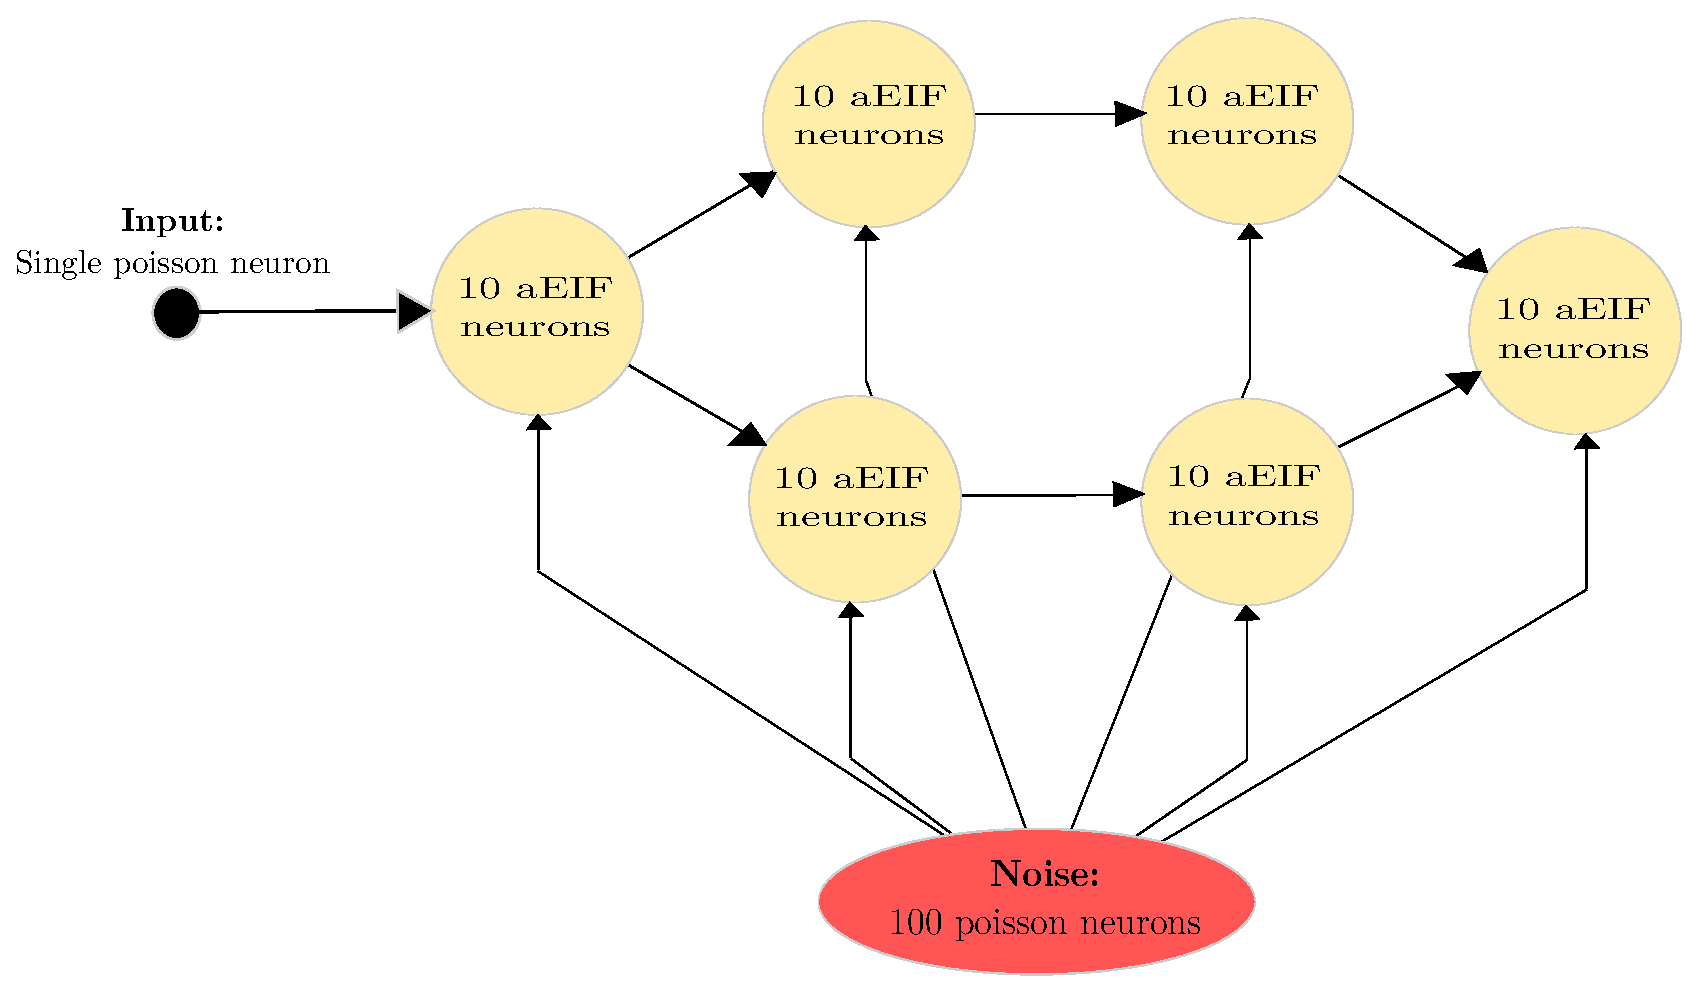
\epsfig{file=modelnetwork.eps, width=20cm}
\vskip 30pt
Our model network is a simple network made up of aEIF neurons \cite{BretteGerstner2006a}, but it has two interesting features, where the network first diverges and then converges.
\vskip 19pt
We chose a connection rate of $0.8$ along the arrows in the network, and overall connection rate of $0.1$ and a rate of $0.2$ from the noise level to the recurrent layer.
\vskip 40pt
\end{textbox}

 \begin{textbox}
 \paragraph{How do these couplings look in our model network?}

 As the image below shows, the directed network is complicated to visualize.  Despite having the network organized in the ``correct'' modules, it is hard to see the modular structure of the network.
\vskip 29pt
\begin{center}
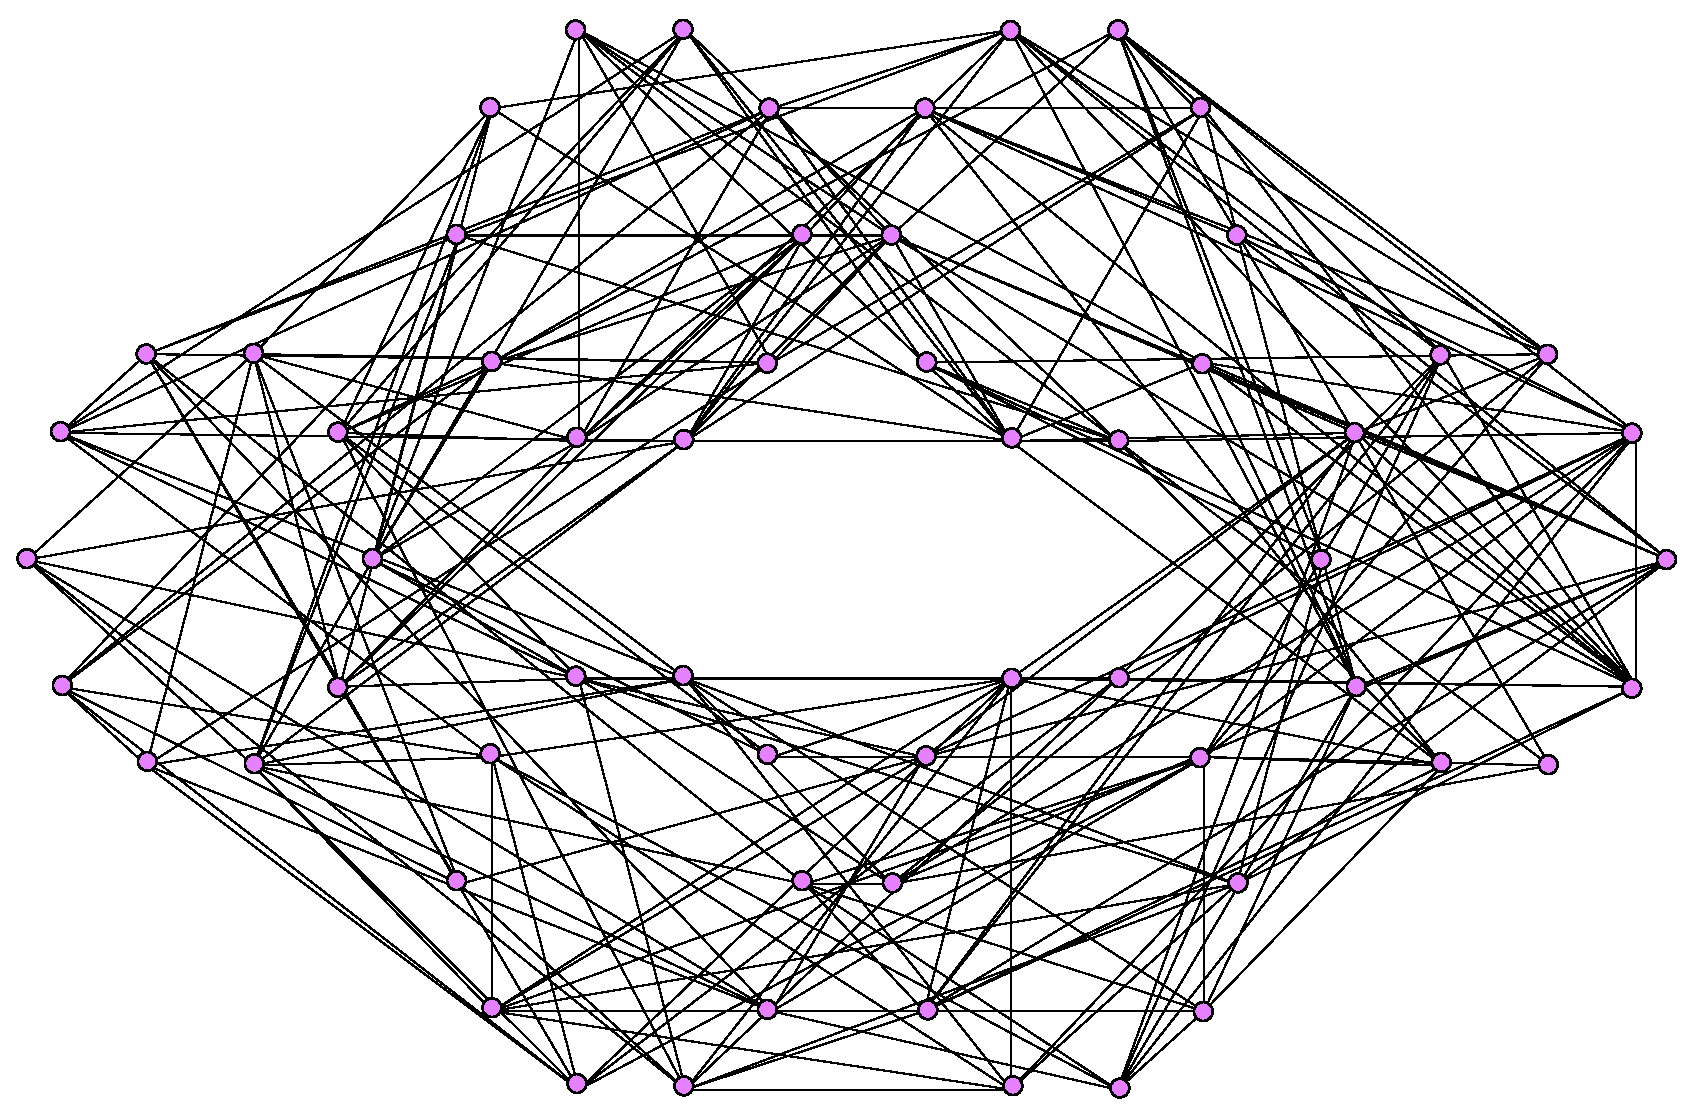
\epsfig{file=directednetnodes.eps, width = 16cm}
\end{center}
\vskip 29pt
First we look at the bibliographic coupling network.
\vskip 29pt
\begin{center}
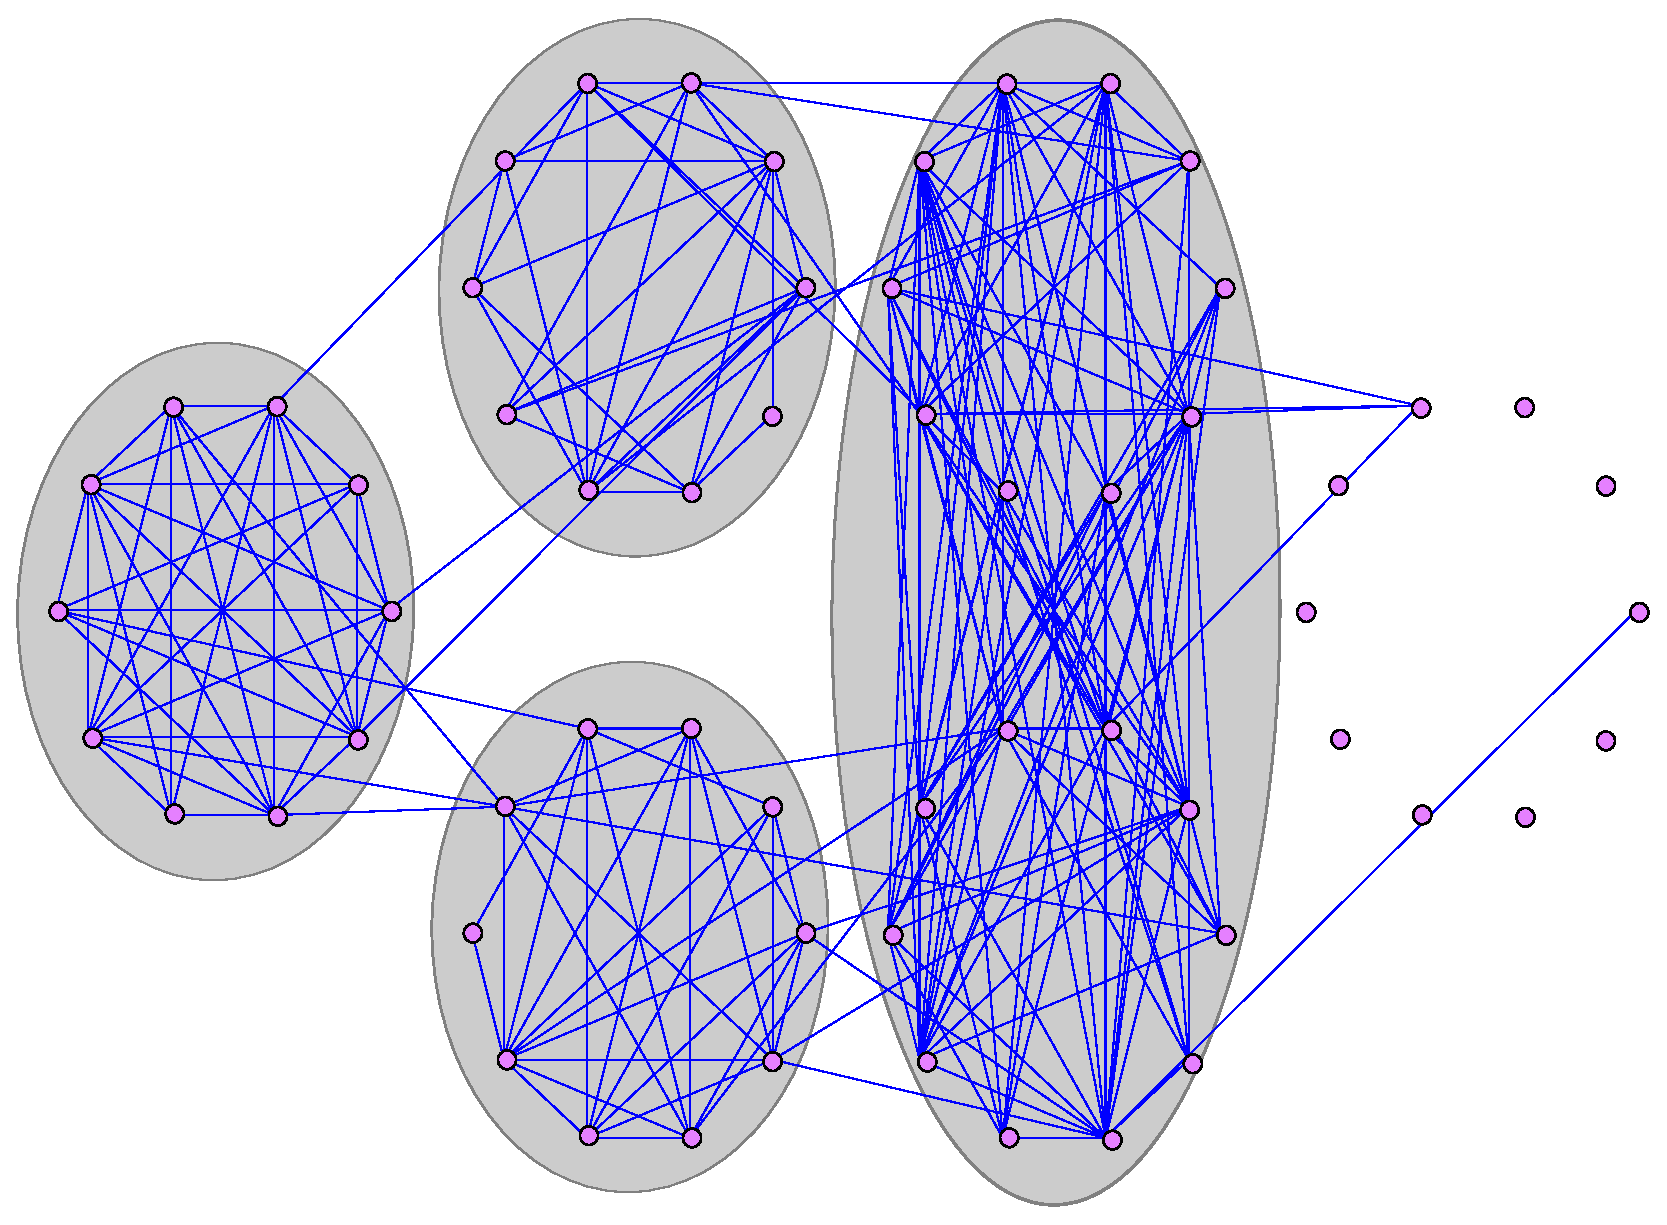
\epsfig{file=clustbibnetnodes.eps, width=16cm}
\end{center}
\vskip 29pt
Above we see the bibliographic coupling network, and its approximate clustering with Newman's clustering algorithm. We see that the bibliographic coupling is very good at detecting a divergence in the network, but is poor at detecting the convergence later in the network.  What about the cocitation coupling?
\vskip 29pt
\begin{center}
 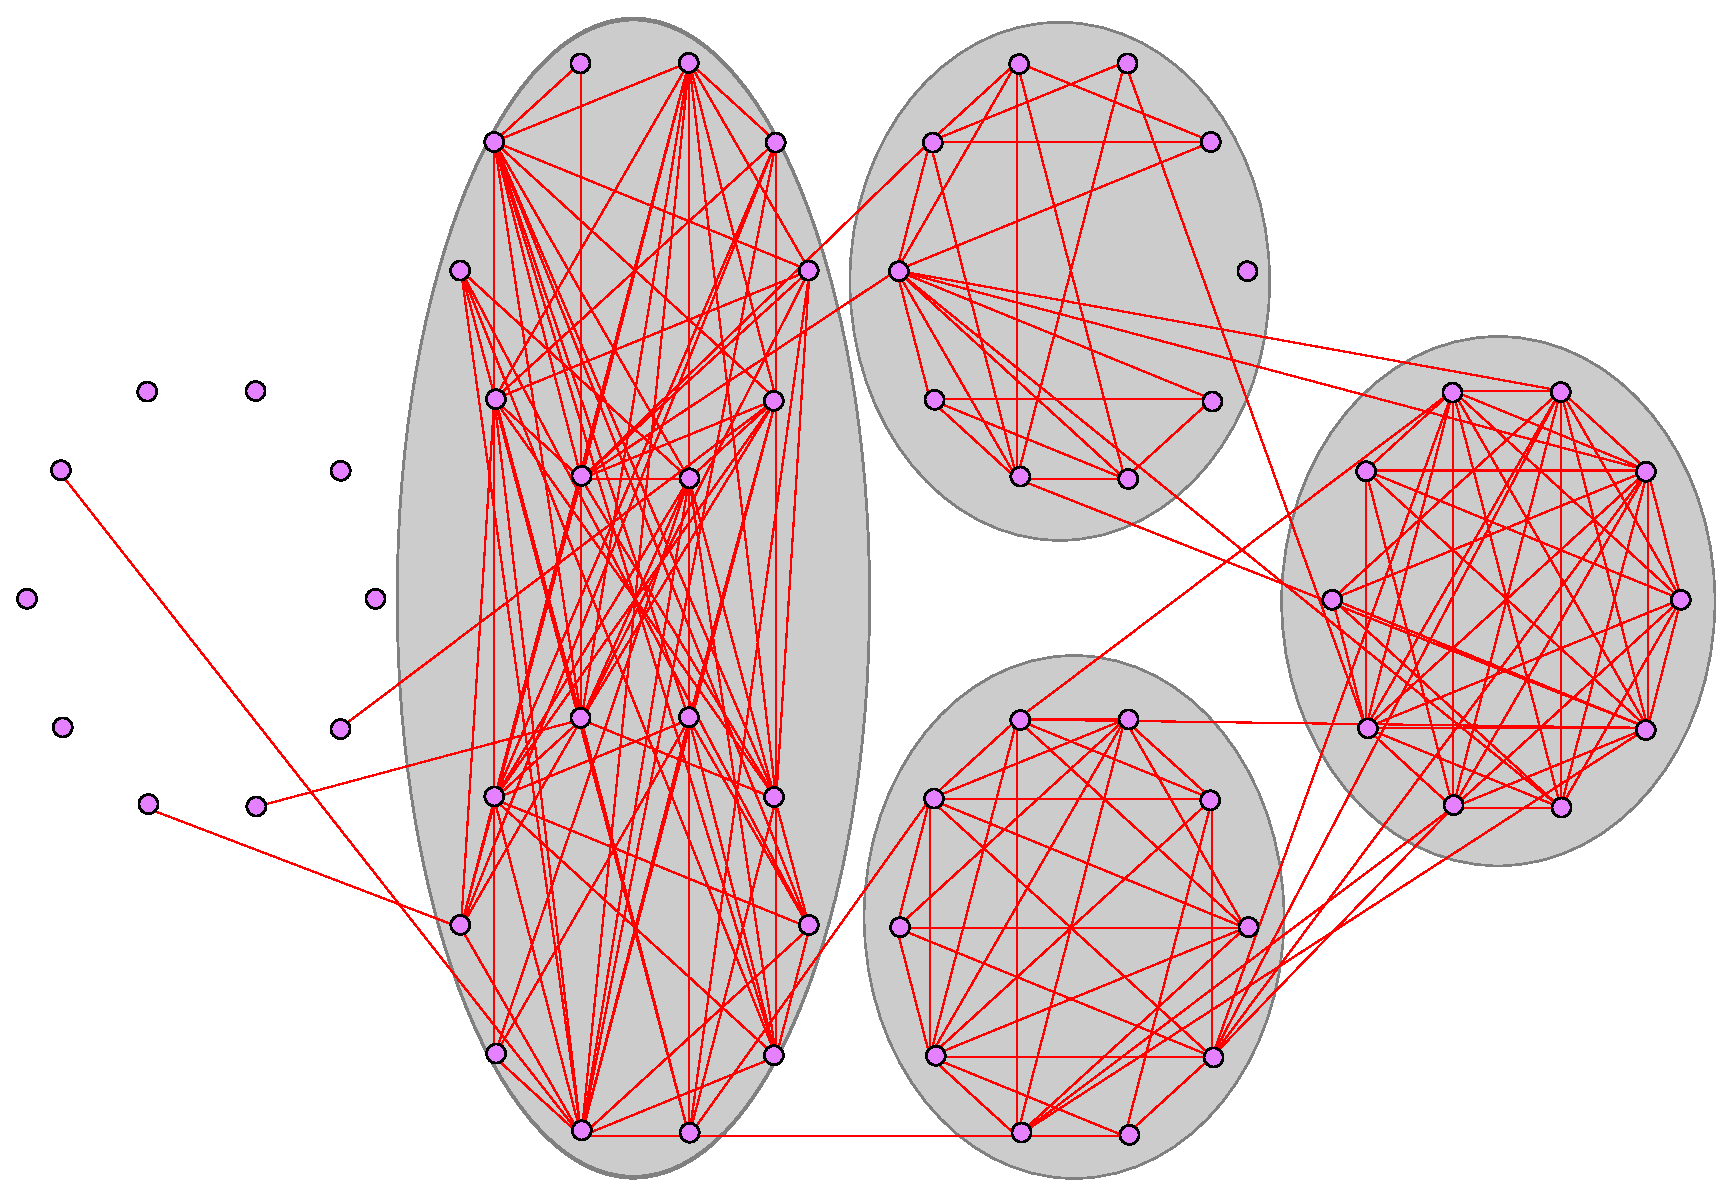
\epsfig{file=clustcocitnetnodes.eps, width = 16cm}
 \end{center}
 \vskip 30pt
 As one might expect, the cocitation coupling exhibits the opposite characteristics, and cannot detect the early divergence in the network, but it does detect the convergence later in the network.
\end{textbox}


}%
%
\col{

\begin{textbox}
\paragraph{Incremental Mutual Information}
\vskip 7pt
The IMI was proposed by Singh and Lesica \cite{SinghLesica2010a}  as a way of characterizing the strength and dynamics of connections in neuronal circuits.  It is a parameter-free measure, that draws its probabilities from observations.

If we have two spike-trains $X$ and $Y$, we first discretize them, then we offset $Y$ by a time-step $\delta$.  Then we compute the mutual information between $X$ and the offset $Y$, dependent on the past and future (for 2/3 time-steps) of both $X$ and $Y$.

Thus the IMI is calculated as: 
$$
\begin{tabular}{lll}
\Delta \mbox{IMI} (\delta)& =  & H(X \left| X_p,X_f,Y(\delta )_p,Y( \delta )_f)  \right. \\
 & - & H(X \left| Y(\delta), X_p,X_f,Y(\delta )_p,Y( \delta )_f) \right.
\end{tabular} 
$$
\end{textbox}

\begin{textbox}
\paragraph{IMI performs better with higher noise levels}
\begin{center}
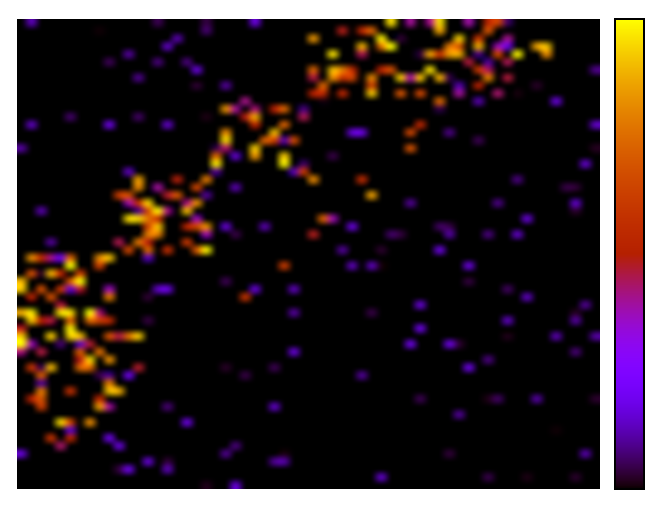
\epsfig{file = weightmatrix.eps, width=12cm}
\end{center}
 The weight matrix of the recurrent network is as shown above.  Below we see how the IMI connections mimic this matrix.
\begin{center}
\begin{tabular}{llll}
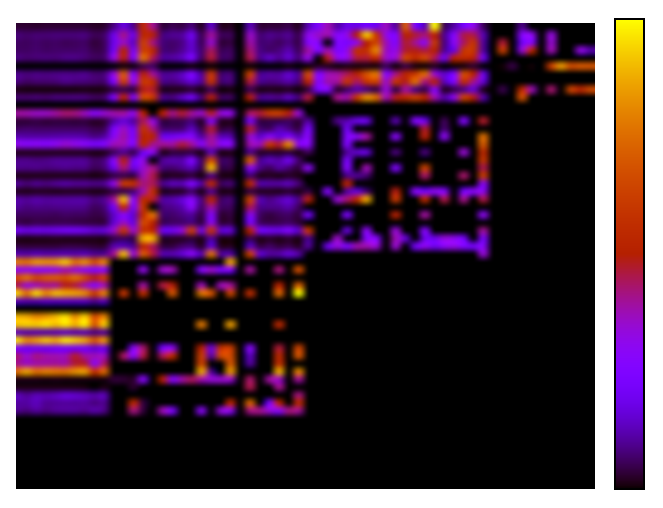
\epsfig{file=IMI1.eps,width=2in} & 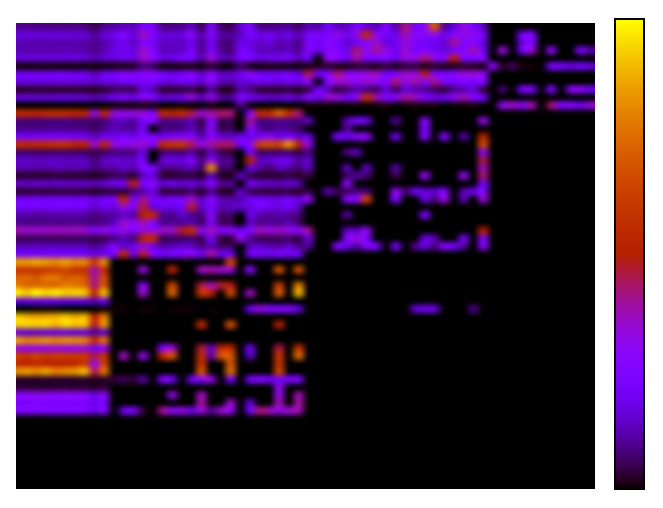
\epsfig{file=IMI2.eps,width=2in} & 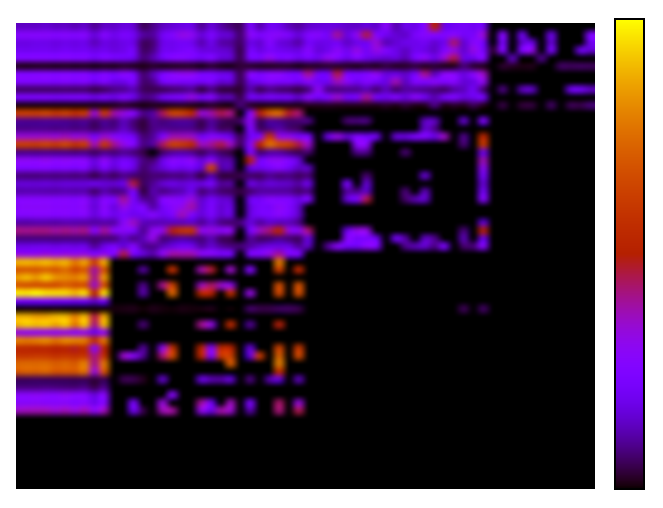
\epsfig{file=IMI3.eps,width=2in} & 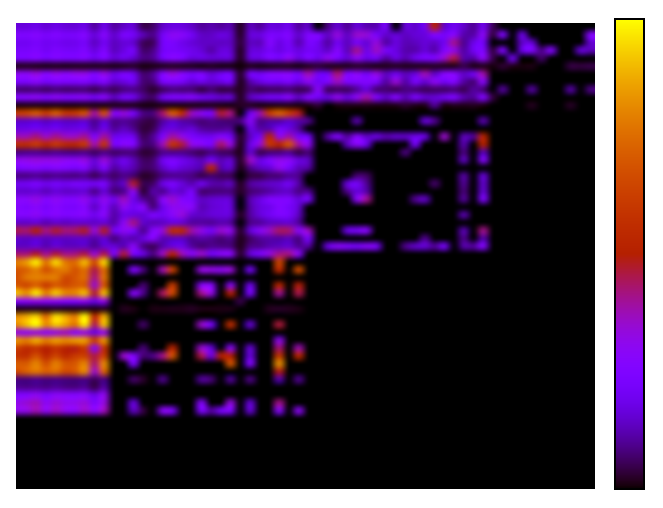
\epsfig{file=IMI4.eps,width=2in} \\
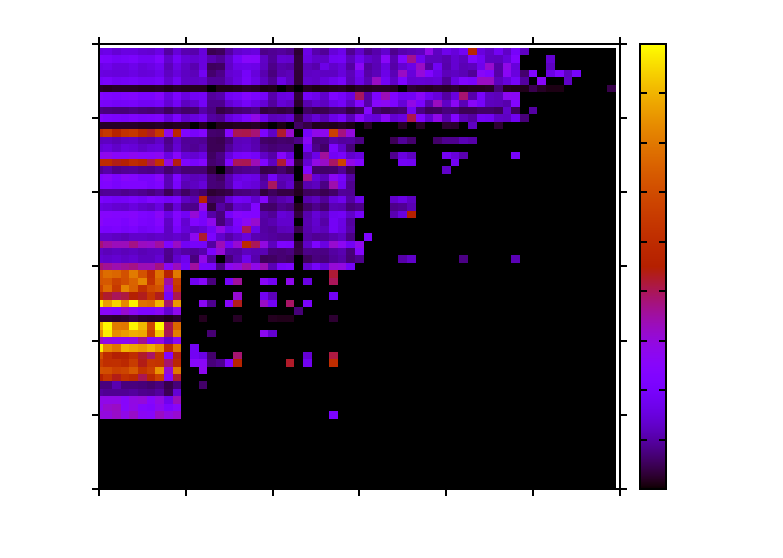
\epsfig{file=IMI5.eps,width=2in} & 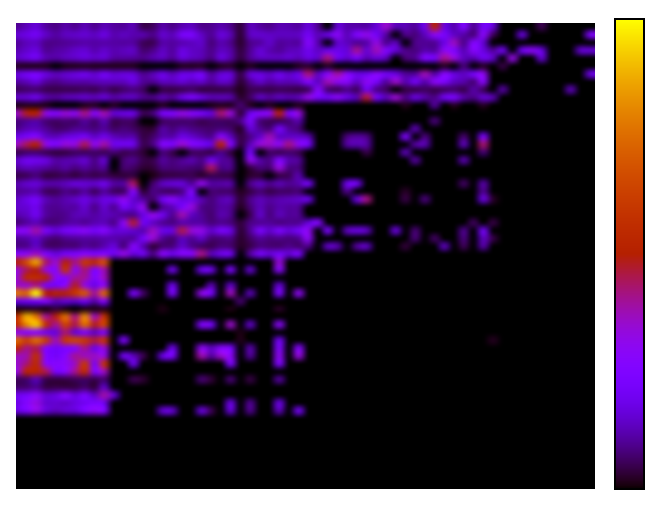
\epsfig{file=IMI6.eps,width=2in} & 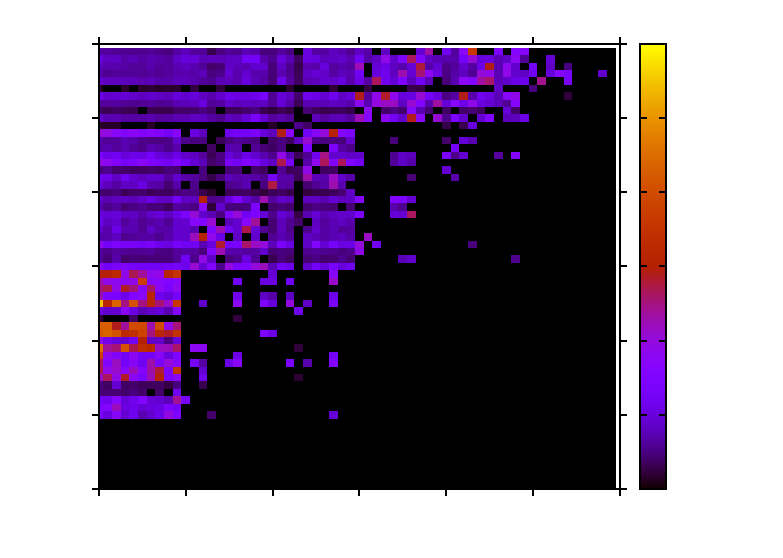
\epsfig{file=IMI7.eps,width=2in} & 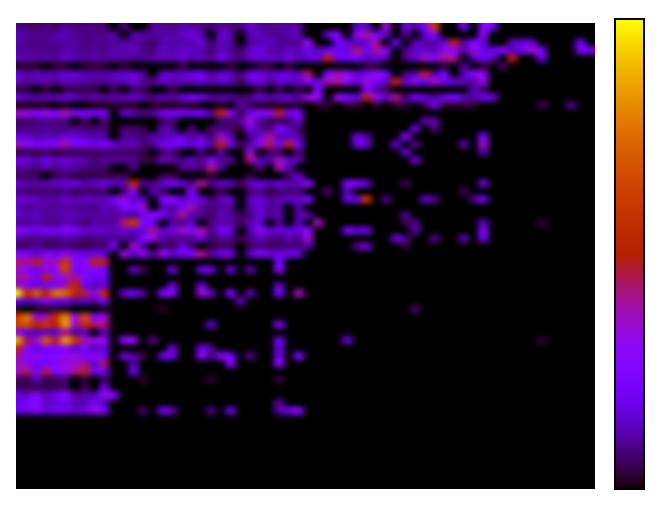
\epsfig{file=IMI8.eps,width=2in} \\
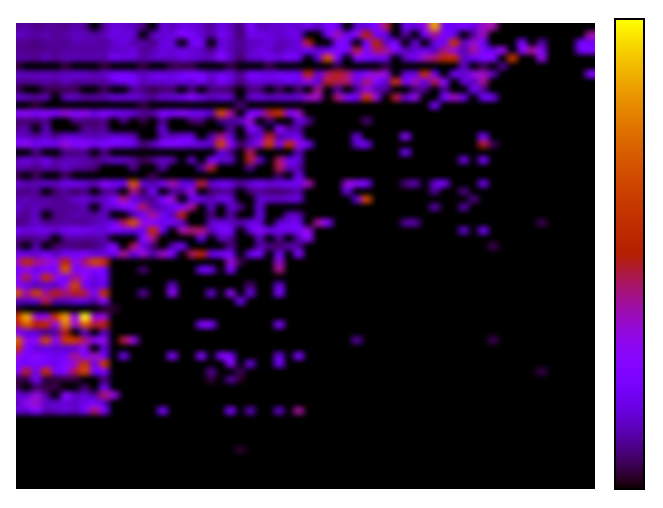
\epsfig{file=IMI9.eps,width=2in} & 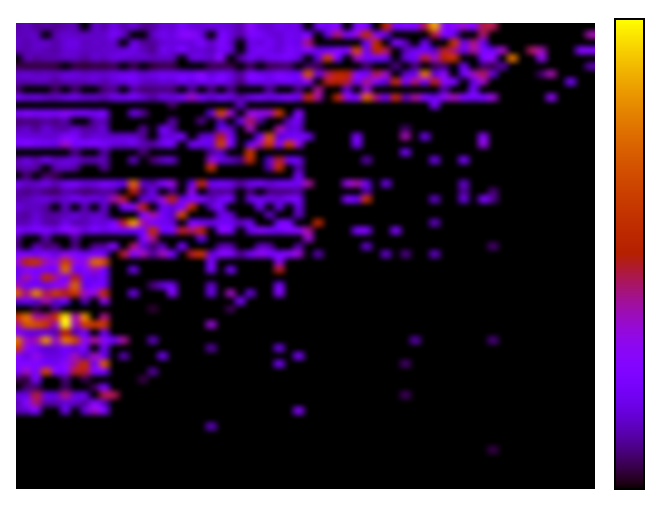
\epsfig{file=IMI10.eps,width=2in} & 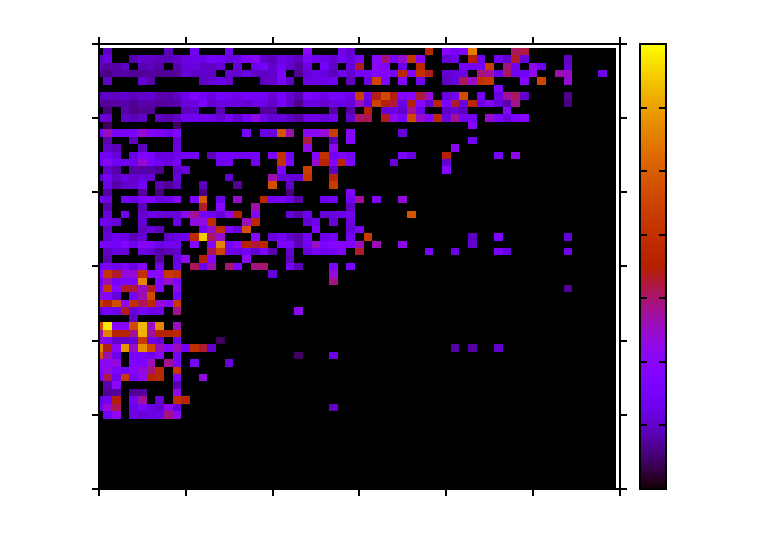
\epsfig{file=IMI11.eps,width=2in} & 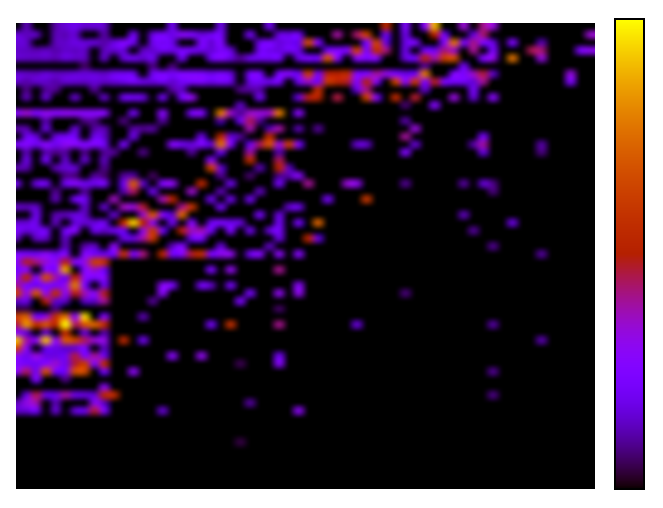
\epsfig{file=IMI12.eps,width=2in}\\
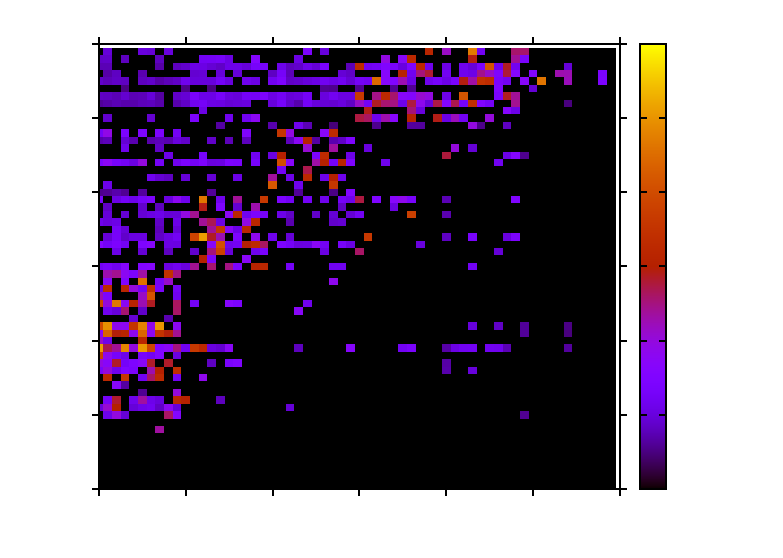
\epsfig{file=IMI13.eps,width=2in} & 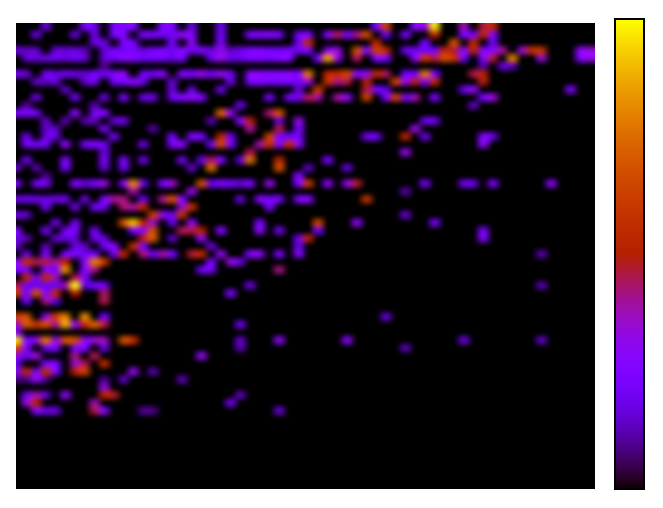
\epsfig{file=IMI14.eps,width=2in} & 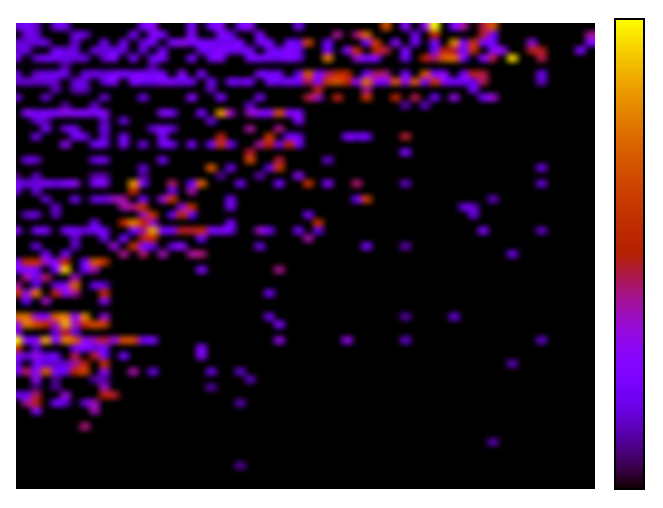
\epsfig{file=IMI15.eps,width=2in} & 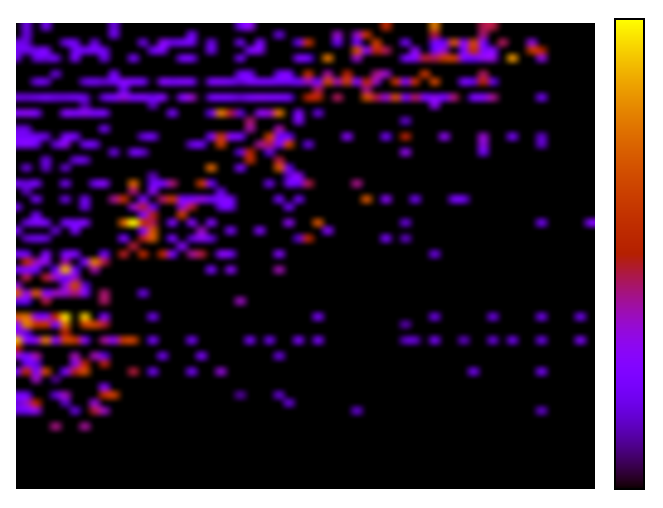
\epsfig{file=IMI16.eps,width=2in}
\end{tabular}
\end{center}
Above are the Incremental Mutual Information matrices of the network as the amplitude of the noise neurons increases from approx. 1 mv to approx. 16 mv.  While the absolute peak IMI values drop as the noise increases, the IMI matrix mimics the actual weight matrix more.

\end{textbox}

\begin{textbox}
\paragraph{Discussion} 
\vskip 7pt
The Incremental Mutual Information is very good at picking out direct influence of neurons on each other, especially when the background noise is high.  Thus, this is a very good tool for analyzing networks of neurons.

The bibliographic and cocitation couplings both pick out important features of the network.  We need to find a way to combine the two clusterings in a consistent manner for this method to be useful.

The method has not been tested on large networks as of yet.

\end{textbox}

\begin{textbox}
{\footnotesize
\begin{thebibliography}{10}

\bibitem{Newman2006a}
Newman M.E.J.
\newblock Modularity and community structure in networks
\newblock {\em PNAS}, vol. 103 : no. 23 : 8577--8582, 2006.

\bibitem{SinghLesica2010a}
Singh A, Lesica N.A.
\newblock Incremental Mutual Information: A New Method for Characterizing the Strength and Dynamics of Connections in Neuronal Circuits
\newblock (\em PNAS), Volume 6, Issue 12, e1001035.

\bibitem{BretteGerstner2006a}
Brette R, Gerstner W.
\newblock {\em Journal of Neurophysiology}, 96:252--258, 2006.

\bibitem{NewmanBook}
Newman, M.E.J.
\newblock {\em Oxford University Press}, Networks pg. 115-118, 2010.


\end{thebibliography}
}
\end{textbox}
}%
\end{center}
\end{document}
